        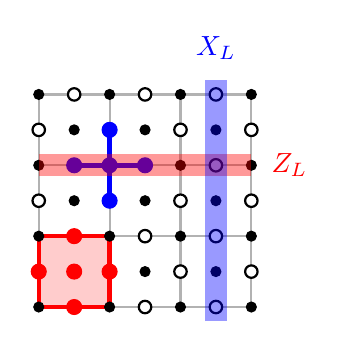
\begin{tikzpicture}[scale=0.9]
            % Draw the main grid lines (the lattice)
            \draw[gray!60, thick] (0,0) grid (3,3);
        
            % Highlight Z-stabilizer (Plaquette)
            % Picked the bottom-left plaquette 
            \filldraw[red!20, draw=red, ultra thick] (0,0) rectangle (1,1);
            
            % Highlight X-stabilizer (Vertex)
            % Picked an internal vertex at (1,2)
            \draw[blue, ultra thick] (0.5,2) -- (1.5,2);
            \draw[blue, ultra thick] (1,1.5) -- (1,2.5);
        
            % Draw ALL Z-ancillas (Faces) as solid black dots
            \foreach \x in {0.5, 1.5, 2.5} {
                \foreach \y in {0.5, 1.5, 2.5} {
                    \filldraw[black] (\x,\y) circle (2pt);
                }
            }
            
            % Draw ALL X-ancillas (Vertices) as solid black dots
            \foreach \x in {0, 1, 2, 3} {
                \foreach \y in {0, 1, 2, 3} {
                    \filldraw[black] (\x,\y) circle (2pt);
                }
            }
        
            % Overwrite the active ancillas with their respective colors (no text)
            \filldraw[blue] (1,2) circle (3pt);
            \filldraw[red] (0.5, 0.5) circle (3pt);
        
            % Draw data qubits on all horizontal edges (white filled circles)
            \foreach \x in {0.5, 1.5, 2.5} {
                \foreach \y in {0, 1, 2, 3} {
                    \filldraw[black, fill=white, thick] (\x,\y) circle (2.5pt);
                }
            }
            % Draw data qubits on all vertical edges (white filled circles)
            \foreach \x in {0, 1, 2, 3} {
                \foreach \y in {0.5, 1.5, 2.5} {
                    \filldraw[black, fill=white, thick] (\x,\y) circle (2.5pt);
                }
            }
        
            % Fill the specific data qubits involved in the highlighted X check to make them pop
            \filldraw[blue] (0.5,2) circle (3pt);
            \filldraw[blue] (1.5,2) circle (3pt);
            \filldraw[blue] (1,1.5) circle (3pt);
            \filldraw[blue] (1,2.5) circle (3pt);
        
            % Fill the specific data qubits involved in the highlighted Z check to make them pop
            \filldraw[red] (0.5,0) circle (3pt);
            \filldraw[red] (0.5,1) circle (3pt);
            \filldraw[red] (0,0.5) circle (3pt);
            \filldraw[red] (1,0.5) circle (3pt);
        
            % Draw Logical Operators (Strings) as OVERLAYS (drawn last)
            % Z_L is a path on the primal lattice (horizontal, lowered to y=2)
            \draw[red, line width=8pt, opacity=0.4] (0, 2) -- (3, 2) node[right, opacity=1, font=\bfseries] {$Z_L$};
            % X_L is a path on the dual lattice (vertical)
            \draw[blue, line width=8pt, opacity=0.4] (2.5, -0.2) -- (2.5, 3.2) node[above, opacity=1, font=\bfseries] {$X_L$};
        \end{tikzpicture}
